\chapter{Konzeptauswahl}\label{chap:concepts}

Da nicht alle im Skript beschriebenen Konzepte zur digitalen Signalverarbeitung behandelt werden k�nnen und die geforderte Signal�bertragung bestimmte Konzepte voraussetzt, musste eine Auswahl getroffen werden. Die folgenden grundlegenden Module sind in jedem Fall notwendig:

\begin{itemize}
	\item Signalgenerator
	\item Modulator
	\item Demodulator
	\item Filter
	\item Datenquelle
\end{itemize}

Aus diesen ist jeweils die jenige Realisierungsm�glichkeit, die am geeignetsten f�r den Anwendungsfall erscheint auszuw�hlen. Dabei sind die Einschr�nkungen der Hardware eines der Hauptkriterien bei der Entscheidungsfindung.

\section{Signalgenerator}\label{sec:concepts:siggen}

F�r den Signalgenerator kommen zwei Konzepte in Frage: Die \textbf{D}irekte \textbf{D}igitale \textbf{S}ynthese (DDS) und der \textbf{CO}ordinate \textbf{R}otation \textbf{DI}gital \textbf{C}omputer (CORDIC).

\section{Modulator}\label{sec:concepts:modulator}

Auch hier bestehen mehrere M�glichkeiten, wenn FSK als Modulation zum Einsatz kommt: Multiplizierer, Multiplexer und Umschaltung der Generatorfrequenz.

\section{Demodulator}\label{sec:concepts:demodulator}

Als Demodulator bei einer FSK-Modulation kommen mehrere Varianten in Betracht: Spektrumanalyse mittels (\textbf{F}ast) \textbf{F}ourier \textbf{T}ransformation (FFT), H�llkurven-Demodulator, Synchronisation auf Tr�ger mittels \textbf{P}hase \textbf{L}ock \textbf{L}oop (PLL), synchroner Demodulator, ...

\section{Filter}\label{sec:concepts:filter}

Es existieren zwei grundlegende Verfahren zur Realisierung von digitalen Filtern: \textbf{F}inite \textbf{I}mpulse \textbf{R}esponse (FIR) und \textbf{I}nfinite \textbf{I}mpulse \textbf{R}esponse (IIR) Filter. Eine m�gliche Implementierung ist in Abb. \ref{fig:diag:linphase}

\begin{figure}[ht]
	\centering
		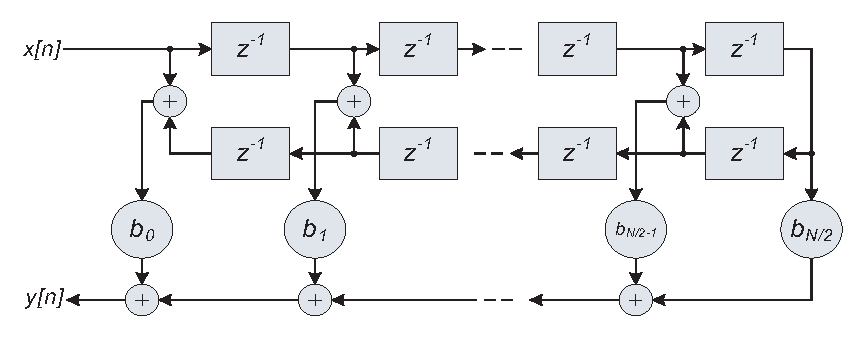
\includegraphics[width=0.70\linewidth]{bilder/FIRLinearphasenstruktur}
	\caption{FIR-Filter in Linearphasenstruktur}
	\label{fig:diag:linphase}
\end{figure}


\section{Datenquelle}\label{sec:concepts:sigsource}

Als Signalquelle bietet sich eine definierte Folge von Werten an. M�gliche Konzepte sind das Auslesen zuvor festgelegter Werte aus einem Speicher und die Erzeugung einer Pseudozufallszahl mittels eines \textbf{P}seudo \textbf{R}andom \textbf{N}oise (PRN, vgl. \ref{fig:diag:prn-shiftreg}) Schieberegisters.

\begin{figure}[ht]
	\centering
		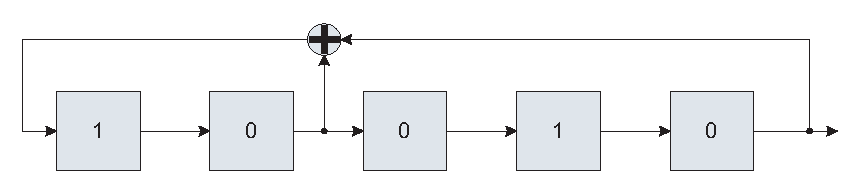
\includegraphics[width=0.70\linewidth]{bilder/prn_register}
	\caption{Schematische Darstellung eines PRN-Schieberegisters}
	\label{fig:diag:prn-shiftreg}
\end{figure}
